%======================================================================
\section{결과}

%----------------------------------------------------------------------
\subsection{그래프의 구조와 덮는 범위}

\begin{yoji}
송금 그래프는 허락 그래프보다 화살표가 2.21배 많아요. 허락 그래프는 많은 주인이 비교적 적은 스펜더를 가리키는 부채 모양이에요. 엔도스랭크는 동점을 거의 남기지 않아요.
\end{yoji}

같은 계약을 두고도 두 그래프는 크기와 모양이 달라요(표~\ref{tab1}).
\begin{itemize}
\item $\Tobs$의 허락 그래프: 점 2,514,846개, 화살표 3,808,949개.
\item $\Tobs$의 송금 그래프: 점 3,603,300개, 화살표 8,426,124개. 화살표가 2.21배 많아요.
\end{itemize}
허락을 거두면 그 화살표가 없어지지만, 기간 중 한 번이라도 송금을 주고받은 쌍에는 송금 화살표가 남아요. 양수의 허락을 가진 주인이 허락 그래프의 점 2,508,872개를 차지해요. 그래서 허락 그래프는 많은 주인이 비교적 적은 스펜더를 가리키는 큰 부채 모양이에요. 양수의 마지막 허락 4,185,287개 가운데 2,084,669개(49.8\%)가 무제한 허락이에요.

코호트를 덮는 범위도 달라요. 코호트 계약 6,483개 가운데 191개는 허락 그래프 밖에 있어요. 기간 안에 그 계약에게 준 허락과 그 계약이 준 허락이 $\Tobs$에 모두 0이었기 때문이에요. 1,192개는 송금 그래프 밖에, 30개는 두 그래프 모두 밖에 있어요. 엔도스랭크는 코호트에서 동점을 거의 남기지 않아요(서로 다른 점수 5,641개, 계약 쌍의 0.20\%가 동점). AWP는 조금 더 남겨요(서로 다른 점수 5,292개, 쌍의 3.38\%가 동점). 동점은 대부분 0점인 계약들 사이에 있어요.

\begin{table}[!htbp]
\centering
\caption{두 동결 시점의 그래프, 그리고 엔도스랭크 닫힌 식의 들어맞음.}
\label{tab1}
\small
\begin{tabular}{@{}L{6.6cm}rr@{}}
\toprule
 & $\Tobs$, 2026년 6월 30일 & $t_1$, 2026년 3월 31일 \\
 & (같은 기간과 W1) & (W0) \\
\midrule
점수 기간 & 2025년 7월 1일 – & 2025년 4월 1일 – \\
 & 2026년 6월 30일 & 2026년 3월 31일 \\
그래프를 둘러싼 코호트 & 6,483(매칭 코호트) & 6,343(W0 코호트) \\
허락 그래프, 점 & 2,514,846 & – \\
허락 그래프, 화살표 & 3,808,949 & 4,117,103$^{a}$ \\
송금 그래프, 점 & 3,603,300 & – \\
송금 그래프, 화살표 & 8,426,124 & 9,198,965$^{a}$ \\
점검한 계약 & 6,483(매칭 코호트) & 7,914(W0 스펜더) \\
그 가운데 스펜더(허락 화살표가 들어옴) & 6,224 & 7,905 \\
\quad 깊이 1(어느 주인에게도 들어오는 화살표가 없음) & 5,232 & 5,092 \\
\quad 더 깊음(주인 가운데 허락을 받은 주소가 있음) & 992 & 2,813 \\
들어오는 화살표가 없는 점의 공통 점수 $c$ & $1.93\times10^{-7}$ & $1.81\times10^{-7}$ \\
닫힌 식$^{b}$과 1\% 안: 깊이 1인 스펜더 & 100.0\% & 100.0\% \\
닫힌 식$^{b}$과 1\% 안: 더 깊은 스펜더 & 21.9\% & 17.8\% \\
닫힌 식$^{b}$과 1\% 안: 모든 스펜더 & 87.5\% & 70.8\% \\
\bottomrule
\end{tabular}

\begin{minipage}{\linewidth}\footnotesize\raggedright\vspace{0.4em}
그래프는 동결마다 그 코호트의 에고 사건을 점수 기간, 곧 동결 직전 12개월에서 모아 만들었어요(수정 분석: WETH, USDC, USDT0, ARB, WBTC의 허락과 송금, 달러 금액). $\Tobs$의 화살표 수는 엔도스랭크나 AWP의 무게가 양수인 쌍의 수예요. 스펜더는 점검한 집합에서 양수 무게의 허락 화살표가 들어오는 계약이고, 그 주인 가운데 누구에게도 들어오는 화살표가 없으면 깊이 1이에요. 감쇠 계수 $d=0.85$. $^{a}$$t_1$의 쌍 표에 있는 주인–스펜더 쌍과 보낸 쪽–받는 쪽 쌍의 수예요. 금액 무게가 부동소수점에서 0이 되는 쌍을 빼기 전에 셌어요. $t_1$의 점 수는 기록하지 않았어요. $^{b}$식~\eqref{eq:closed-form}(\ref{sec:closed}절). 출처: \texttt{revised-usd-12m}의 \texttt{same-window}와 \texttt{holdout-w0/eval\_summary.json}(키 \texttt{graph}, \texttt{closed\_form}, \texttt{analysis/closed-form/closed\_form\_check.json}을 거쳐), \texttt{cohort/matched\_cohort.json}, \texttt{cohort\_t1.json}.
\end{minipage}
\end{table}

%----------------------------------------------------------------------
\subsection{각 점수는 자기 화살표의 점검과 가장 잘 맞아요}

\begin{yoji}
같은 기간에서 엔도스랭크는 허락 가족과, AWP는 송금 가족과 가장 잘 맞았어요. 만든 방식 때문에 예상되는 결과이고, 얼마쯤은 저절로 생긴 일치예요. 두 걷기는 계약을 꽤 다르게 줄 세워요($\tau_b=0.199$).
\end{yoji}

같은 기간에서 각 점수는 자기가 걷는 화살표를 따라가요(표~\ref{tab2}).
\begin{itemize}
\item 허락 가족: 엔도스랭크 $\tau=0.560$ [0.548, 0.571], AWP 0.226 [0.210, 0.245].
\item 송금 가족: AWP 0.736 [0.728, 0.744], 엔도스랭크 0.196 [0.180, 0.216].
\end{itemize}
짝지은 차이는 $\dt=+0.333$ [0.311, 0.354](엔도스랭크 − AWP, 허락 가족)와 +0.539 [0.518, 0.560](AWP − 엔도스랭크, 송금 가족)이에요. 의도한 구성개념 점검이 예상하는 모양이고, 그 일부는 저절로 생겨요. 엔도스랭크는 자기가 다듬는 수인 받은 허락 수와 가장 잘 맞아요(0.650 [0.639, 0.661]).

달러 금액을 쓰니, 받은 송금의 금액과 AWP의 일치(0.730 [0.720, 0.740])가 서로 다른 보낸 쪽 수와의 일치(0.742 [0.732, 0.752])에 가까워요. AWP의 금액 무게가 노리는 대로예요. 시빌 안정성 가족은 계약이 얼마나 오래, 얼마나 고르게 송금을 받아 왔는지를 재는 송금 기반 지표의 평균이에요. 여기서 AWP는 0.419 [0.408, 0.434]에 이르지만, 엔도스랭크는 0.026 [0.012, 0.041]뿐이에요.

활동 재시작을 쓰면 엔도스랭크는 자기 가족(0.601 [0.590, 0.613])과도, 송금 가족(0.251 [0.233, 0.271])과도 더 잘 맞아요. 이때 다시 출발이 대부분 허락을 가장 많이 주는 주인에게 떨어지므로, 스펜더의 점수가 주인이 몇 명인지뿐 아니라 그 주인들이 얼마나 바쁜지에도 달리기 때문이에요.

\begin{table}[!htbp]
\centering
\caption{같은 기간에서 각 점수와 각 화살표 종류의 점검의 일치(의도한 구성개념 점검).}
\label{tab2}
\small
\begin{tabular}{@{}lccc@{}}
\toprule
점검(켄달의 $\tau_b$ [95\% 구간]) & EndorseRank & \begin{tabular}[b]{@{}c@{}}EndorseRank,\\ 활동 재시작\end{tabular} & AWP \\
\midrule
송금 가족(평균) & 0.196 [0.180, 0.216] & 0.251 [0.233, 0.271] & 0.736 [0.728, 0.744] \\
\quad 입차수 & 0.218 [0.199, 0.238] & 0.272 [0.252, 0.292] & 0.742 [0.732, 0.752] \\
\quad 받은 금액(달러) & 0.175 [0.157, 0.194] & 0.231 [0.213, 0.251] & 0.730 [0.720, 0.740] \\
허락 가족(평균) & 0.560 [0.548, 0.571] & 0.601 [0.590, 0.613] & 0.226 [0.210, 0.245] \\
\quad 받은 허락 수 & 0.650 [0.639, 0.661] & 0.669 [0.659, 0.680] & 0.242 [0.223, 0.262] \\
\quad 받은 허락 금액(달러, 상한) & 0.469 [0.454, 0.484] & 0.534 [0.520, 0.549] & 0.211 [0.193, 0.229] \\
시빌 안정성 가족(평균) & 0.026 [0.012, 0.041] & 0.056 [0.042, 0.072] & 0.419 [0.408, 0.434] \\
\midrule
\multicolumn{4}{@{}l}{\emph{짝지은 차이 $\dt$ [95\% 구간]과 두 순위의 일치}} \\
EndorseRank − AWP, 허락 가족 & \multicolumn{3}{l}{+0.333 [0.311, 0.354]} \\
AWP − EndorseRank, 송금 가족 & \multicolumn{3}{l}{+0.539 [0.518, 0.560]} \\
EndorseRank와 AWP 사이의 $\tau_b$ & \multicolumn{3}{l}{0.199 [0.181, 0.221]} \\
\quad 빠진 계약을 외톨이 점으로 넣으면 & \multicolumn{3}{l}{0.199 [0.181, 0.221]} \\
\bottomrule
\end{tabular}

\begin{minipage}{\linewidth}\footnotesize\raggedright\vspace{0.4em}
매칭 코호트 $n=6{,}483$ 계약, $\Tobs$(2026년 6월 30일)의 점수, 점수 기간은 2025년 7월 1일부터 2026년 6월 30일까지이고 점검도 같은 기간에서 계산했어요. 각 점검은 한 그래프의 사건에서 계산해요. 송금 가족은 받은 송금에서, 허락 가족은 받은 마지막 허락에서 와요. 그래서 점수가 자기 화살표 종류의 점검과 맞는 것은 얼마쯤 저절로 생겨요. 시빌 안정성 가족은 받은 상대의 비율, 송금 기간, 활동한 달 수의 평균이에요. 가족 평균은 그 점검들의 계수를 그냥 평균한 값이에요. 짝지은 계약 부트스트랩 400번(시드 42), 보정하지 않은 구간. 이 비교 가운데 어느 것도 규칙을 판정하지 않아요. 출처: \texttt{revised-usd-12m/same-window/eval\_summary.json}의 \texttt{families}, \texttt{per\_proxy}, \texttt{contrasts}, \texttt{inter\_method}.
\end{minipage}
\end{table}

두 걷기는 계약을 다르게 줄 세워요. 두 순위의 일치는 $\tau_b=0.199$ [0.181, 0.221]이에요. 코호트 계약의 쌍 21,011,403개 가운데 두 점수가 모두 순서를 정하는 쌍이 96.4\%이고, 그 가운데 39.8\%에서 두 점수의 방향이 엇갈려요. 그래프 밖의 계약을 외톨이 점으로 넣어도(계획이 정한 민감도 분석) 이 일치는 보고한 소수 셋째 자리까지 바뀌지 않아요. 송금 기반 점수에 기대는 프로토콜은, 허락 기반 점수로 바꿔도 계약의 순서가 그대로 남으리라고 가정할 수 없어요.

\begin{puri}[자기 화살표의 점검과 맞는 것이 왜 “저절로”인가요?]
엔도스랭크는 허락 화살표로 만들고, 허락 가족도 같은 허락 화살표로 세요. 같은 재료로 만든 두 값이 비슷하게 줄 서는 것은 당연해요. 그래서 표~\ref{tab2}는 “각 점수가 재려는 것을 재고 있다”는 확인일 뿐, 점수가 앞일을 맞힌다는 증거가 아니에요. 다음 절은 동결 뒤의 자료로 시험해요. 다만 그 라벨도 같은 종류의 나중 화살표라서, 그 시험이 보여 주는 것은 구성개념이 이어진다는 것(지속성)이에요. 다른 종류의 결과는 트레이더 비교(\ref{sec:neutral}절)에서 봐요.
\end{puri}

%----------------------------------------------------------------------
\subsection{기간 밖: 각 화살표 종류는 같은 종류의 나중 화살표를 줄 세워요}

\begin{yoji}
동결 뒤 석 달 동안, 허락으로 만든 점수는 새 허락 쌍을, 송금으로 만든 점수는 새 송금자를 더 잘 줄 세웠어요. 두 창 모두에서 같은 화살표 종류의 원시 차수가 가장 앞섰어요.
\end{yoji}

표~\ref{tab3}은 각 날짜에 동결한 모든 점수를 두 스펜더 라벨과 견줘요. 지속성에서 예상하듯, 화살표 종류가 어느 라벨을 가장 잘 줄 세울지를 정해요.
\begin{itemize}
\item \textbf{W0, 새 허락 쌍:} 받은 허락 수 $\tau=0.392$ [0.377, 0.406], 엔도스랭크 0.303 [0.287, 0.319], 그 활동 변형 0.332 [0.315, 0.347]. 송금 입차수(0.203 [0.183, 0.224])와 AWP(0.196 [0.178, 0.213])는 더 낮아요.
\item \textbf{W0, 새 송금자:} 순서가 뒤집혀요. 송금 입차수 0.447 [0.435, 0.459], AWP 0.409 [0.396, 0.421], 엔도스랭크 0.272 [0.257, 0.286].
\item 엔도스랭크 − AWP는 새 허락 쌍에서 $\dt=+0.107$ [0.086, 0.130], 새 송금자에서 −0.138 [−0.151, −0.123]이에요.
\item \textbf{W1}도 같은 모양이에요. 엔도스랭크 − AWP는 새 허락 쌍에서 +0.142 [0.119, 0.164], 새 송금자에서 −0.139 [−0.154, −0.125]예요.
\end{itemize}
두 창 모두에서 같은 화살표 종류의 수가 자기 라벨에서 앞서요.

\begin{table}[!htbp]
\centering
\caption{스펜더 홀드아웃: 각 날짜에 동결한 점수와 그 뒤 석 달 동안 센 라벨.}
\label{tab3}
\footnotesize
\setlength{\tabcolsep}{1.5pt}
\begin{tabular}{@{}L{3.1cm}cccc@{}}
\toprule
 & \multicolumn{2}{c}{W0: 2026년 3월 31일 동결($n=7{,}914$)} & \multicolumn{2}{c}{W1: 2026년 6월 30일 동결($n=7{,}960$)} \\
\cmidrule(lr){2-3}\cmidrule(lr){4-5}
동결 시점의 점수 & 새 허락 쌍 & 새 송금자 & 새 허락 쌍 & 새 송금자 \\
\midrule
받은 허락 수(셈) & 0.392 [0.377, 0.406] & 0.284 [0.267, 0.299] & 0.381 [0.365, 0.396] & 0.269 [0.250, 0.285] \\
송금 입차수(셈) & 0.203 [0.183, 0.224] & 0.447 [0.435, 0.459] & 0.165 [0.143, 0.186] & 0.439 [0.426, 0.454] \\
EndorseRank & 0.303 [0.287, 0.319] & 0.272 [0.257, 0.286] & 0.299 [0.284, 0.314] & 0.259 [0.243, 0.275] \\
EndorseRank, 활동 재시작 & 0.332 [0.315, 0.347] & 0.270 [0.256, 0.285] & 0.335 [0.319, 0.349] & 0.236 [0.219, 0.251] \\
AWP & 0.196 [0.178, 0.213] & 0.409 [0.396, 0.421] & 0.157 [0.137, 0.178] & 0.398 [0.386, 0.412] \\
\midrule
\multicolumn{5}{@{}l}{\emph{각 페이지랭크 − 그것이 다듬는 원시 차수, 자기 화살표 종류의 라벨에서: $\dt$ [95\% 구간]}} \\
EndorseRank − 받은 허락 수 & −0.090 [−0.100, −0.079] & & −0.082 [−0.090, −0.073] & \\
EndorseRank, 활동 재시작 − 받은 허락 수 & −0.060 [−0.070, −0.052] & & −0.046 [−0.055, −0.038] & \\
AWP − 송금 입차수 & & −0.038 [−0.043, −0.032] & & −0.041 [−0.047, −0.034] \\
\multicolumn{5}{@{}l}{\emph{허락 걷기 대 송금 걷기: $\dt$ [95\% 구간]}} \\
EndorseRank − AWP & +0.107 [0.086, 0.130] & −0.138 [−0.151, −0.123] & +0.142 [0.119, 0.164] & −0.139 [−0.154, −0.125] \\
\bottomrule
\end{tabular}

\begin{minipage}{\linewidth}\footnotesize\raggedright\vspace{0.4em}
켄달의 $\tau_b$와 95\% 백분위 구간(짝지은 계약 다시 뽑기 400번, 시드 42). 구간은 보정하지 않았어요. 스펜더는 점수 기간에 정한, 다섯 토큰 가운데 하나의 양수 마지막 허락을 동결 시점에 가진 계약이에요. W0에서는 1,732개가 새 허락 쌍을, 1,422개가 새 송금자를 하나 이상 얻었고, W1에서는 1,495개와 1,371개가 얻었어요. 이 표의 짝지은 차이는 모두 그 창의 라벨을 안 뒤에 계산했고, 어느 것도 규칙을 판정하지 않아요. 출처: \texttt{revised-usd-12m/holdout-w0/eval\_summary.json}(\texttt{taus}, \texttt{contrasts\_after}), \texttt{window-w1/eval\_summary.json}(\texttt{spender\_taus}, \texttt{endorserank\_results}), \texttt{supplementary/supplementary.json}.
\end{minipage}
\end{table}

\begin{puri}[표~\ref{tab3}은 어떻게 읽나요?]
위의 다섯 줄은 점수마다 라벨을 얼마나 잘 줄 세웠는지($\tau_b$)예요. 같은 열 안에서 수가 큰 점수가 그 라벨을 더 잘 줄 세운 거예요. W0의 새 허락 쌍 열에서는 받은 허락 수(0.392)가, 새 송금자 열에서는 송금 입차수(0.447)가 가장 커요. 아래 줄들은 두 점수의 짝지은 차이예요. 페이지랭크 − 원시 차수의 차이가 모두 음수라는 것이 다음 절의 결과예요.
\end{puri}

%----------------------------------------------------------------------
\subsection{어느 걷기도 자기가 다듬는 원시 차수를 넘지 못했어요}

\begin{yoji}
자기 화살표 종류의 라벨에서 AWP는 송금 입차수보다, 엔도스랭크는 받은 허락 수보다 두 창 모두 낮았어요. 활동 재시작은 간격을 좁혔지만 메우지 못했어요. 이 비교는 모두 라벨을 안 뒤에 계산했어요.
\end{yoji}

자기 화살표 종류의 라벨에서, 어느 걷기도 자기가 다듬는 원시 차수보다 낫지 않았어요(그림~\ref{fig1}A).
\begin{itemize}
\item \textbf{AWP:} 나중의 새 송금자에서 AWP는 송금 입차수보다 W0에서 $\dt=-0.038$ [−0.043, −0.032], W1에서 −0.041 [−0.047, −0.034] 뒤져요. 송금 쪽에서, 시간 무게와 금액 무게와 활발한 송금자에서의 다시 출발을 다 갖춘 AWP의 걷기가, 새로 들어온 송금자의 수를 서로 다른 보낸 쪽의 수만큼 잘 줄 세우지 못한 거예요.
\item \textbf{엔도스랭크:} 계획대로 고르게 다시 출발하는 엔도스랭크는 나중의 새 허락 쌍에서 받은 허락 수보다 W0에서 −0.090 [−0.100, −0.079], W1에서 −0.082 [−0.090, −0.073] 뒤져요.
\end{itemize}
양쪽 모두 서로 다른 상대의 수가 더 나은 예측 지표였어요. 계획도 등록 문서도 이 대비를 하나도 이름 붙이지 않았어요. 등록 분석에서는, 등록과 함께 커밋한 평가 코드에 엔도스랭크와 AWP를 각자의 차수와 견주는 W1 대비 둘이 이미 들어 있었어요. 이 연구가 W1 로그를 추출하기 전이에요. W0 대비, 활동 변형의 대비, 그리고 수정 분석의 모든 대비는 라벨을 안 뒤에 고르고 계산했어요.

\begin{figure}[!htbp]
\centering
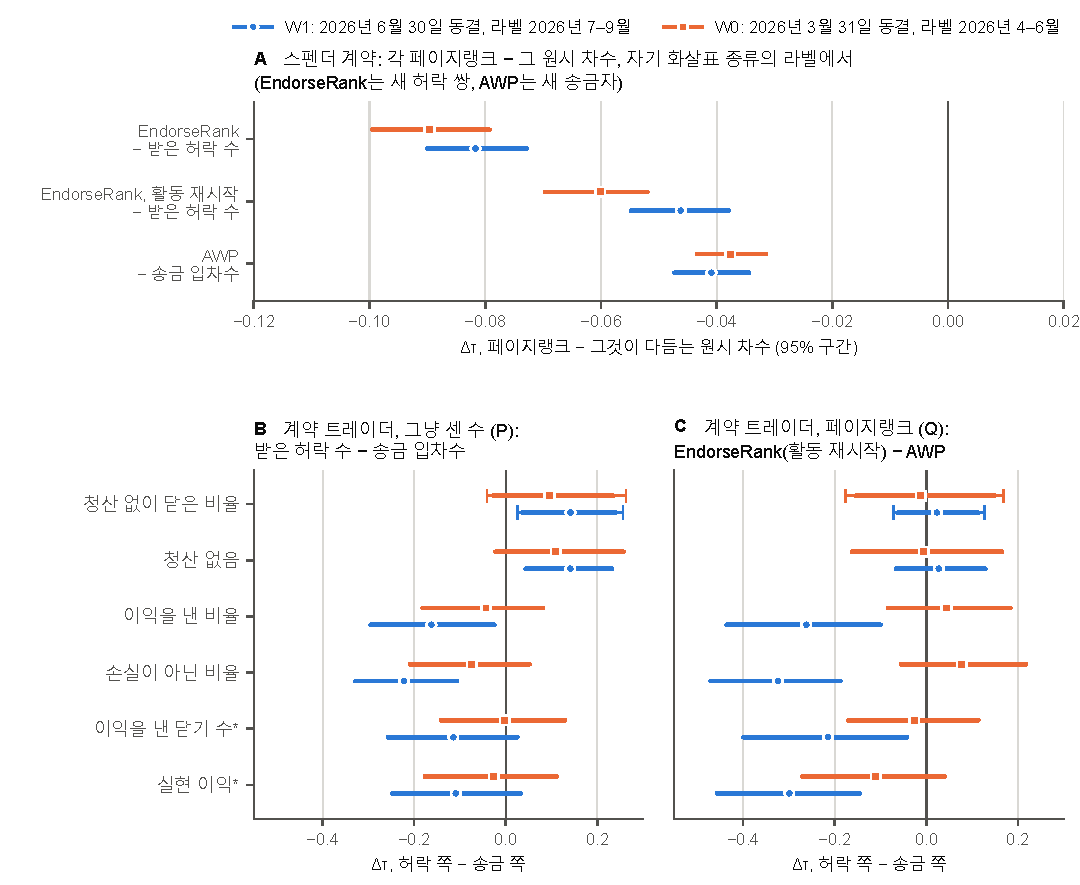
\includegraphics[width=\linewidth]{figures/fig1_ko.pdf}
\caption[페이지랭크 대 원시 차수(스펜더 계약), 허락 쪽 대 송금 쪽(계약 트레이더).]{\textbf{페이지랭크 대 원시 차수(스펜더 계약), 허락 쪽 대 송금 쪽(계약 트레이더).} 점마다 석 달 라벨 기간이 시작할 때 동결한 두 점수의 켄달 $\tau_b$ 짝지은 차이예요. 파란 동그라미는 W1(2026년 6월 30일 동결, 라벨 2026년 7–9월), 주황 네모는 W0(2026년 3월 31일 동결, 라벨 2026년 4–6월)이에요. 굵은 선은 보정하지 않은 95\% 짝지은 부트스트랩 구간이에요. (A) 스펜더 계약(W0 $n=7{,}914$, W1 $7{,}960$; 다시 뽑기 400번): 각 페이지랭크 − 그것이 다듬는 원시 차수. 엔도스랭크 두 변형은 새 허락 쌍에서, AWP는 새 송금자에서 견줬고, 라벨을 안 뒤에 계산했어요. (B) 계약 트레이더(W0 $n=87$, W1 $70$; 다시 뽑기 2,000번): 받은 허락 수 − 송금 입차수(대비 P)를 나중 결과 여섯 개에서. (C) 같은 것을 활동 재시작 엔도스랭크 − AWP(대비 Q)로. (B)와 (C)의 첫 줄에서 끝 눈금이 있는 가는 선은 97.5\% 구간이에요. W1에서는 이것이 등록 규칙의 판정 구간이고, 여기서는 수정 점수에 적용했어요. 별표는 닫기 수에 따라 커지는 두 결과예요. 수정 분석(달러 금액, 다섯 토큰, 동결 직전 12개월의 점수).}
\label{fig1}
\end{figure}

\paragraph{활동 재시작.}
AWP의 활동 재시작을 쓰면, 엔도스랭크는 두 창 모두에서 새 허락 쌍을 균등 재시작 꼴보다 잘 줄 세워요. W0에서 +0.029 [0.023, 0.037], W1에서 +0.035 [0.029, 0.042]만큼이에요. 그래도 여전히 받은 허락 수보다는 낮아요(−0.060 [−0.070, −0.052]와 −0.046 [−0.055, −0.038]). 두 변형은 걷기가 어디서 다시 출발하는지만 달라요. 그러니 이 라벨에서 활동 재시작은 수와의 간격을 좁히지만 메우지는 못해요. 이 비교도 각 창의 라벨을 안 뒤에 했어요.

\paragraph{덮는 범위.}
덮는 범위로는 차수 비교를 설명할 수 없어요. AWP는 동결 전에 송금 화살표가 없던 W0 스펜더 1,342개, 곧 약 6개 가운데 1개에 0점을 줘요. 이 스펜더들은 나중에 새 허락 쌍은 다른 스펜더보다 더 자주 얻었지만(26.7\% 대 20.9\%), 새 송금자는 거의 얻지 못했어요(1.4\% 대 21.3\%). 동결 전에 다른 주소에게서 송금을 받은 스펜더 6,489개로 좁혀도(결과를 안 뒤에 고른 부분 집합), 두 차수 비교의 부호는 그대로예요. AWP − 송금 입차수는 새 송금자에서 −0.051 [−0.059, −0.043], 엔도스랭크 − 받은 허락 수는 새 허락 쌍에서 −0.087 [−0.096, −0.078]이에요.

하지만 덮는 범위가 화살표 종류 사이의 비교는 얼마쯤 설명해요. 그 부분 집합에서 AWP는 새 허락 쌍을 0.328 [0.312, 0.343]으로 줄 세워요. 엔도스랭크(0.299 [0.283, 0.315])보다 위이고 받은 허락 수(0.387 [0.370, 0.402])보다 아래예요. 짝지은 대비는 계산하지 않았어요. 그러니 새 허락 쌍에서 엔도스랭크가 AWP보다 앞선 것은 그 부분 집합 밖의 스펜더에서 와요. AWP가 0점을 준 1,342개가 여기에 들어가요.

\paragraph{동점.}
동점도 양쪽에서 한몫할 수 있어요. 받은 허락 수와 송금 입차수는 동점이 아주 많은 정수예요. 엔도스랭크는 W0 스펜더 7,914개에 서로 다른 점수 7,368개를 주고, 쌍의 0.058\%만 동점이에요. AWP는 그 가운데 1,342개에 똑같이 0점을 주고, 쌍의 2.87\%가 동점이에요. $\tau_b$는 이 둘을 다르게 다루는데, 동점에 흔들리지 않는 비교는 하지 않았어요.

\paragraph{다른 두 라벨.}
계획이 정하지 않은 라벨 두 개를 W0 스펜더에서 더 계산했어요.
\begin{itemize}
\item \textbf{허락 거두기:} 동결 시점에 양수의 허락을 둔 주인 가운데, 라벨 기간에 그 허락을 0으로 바꾼 주인의 수.
\item \textbf{털린 주인:} 새 허락 뒤 몇 시간 안에 같은 토큰이 밖으로 송금된 주인의 수. 휴리스틱으로 세요(S1 Text).
\end{itemize}
모든 점수가 두 라벨을 양의 방향으로 줄 세워요. 허락 거두기는 받은 허락 수를 가장 잘 따르고(0.384 [0.366, 0.399]), 송금 입차수를 가장 못 따라요(0.186 [0.167, 0.209]). 털린 주인의 계수는 송금 입차수의 0.162 [0.143, 0.183]부터 활동 재시작 엔도스랭크의 0.341 [0.325, 0.356]까지예요. 주인들이 더 믿은 계약이라면 허락을 더 자주가 아니라 덜 자주 잃어야 해요. 그러니 이 수들은 보증보다는 주인 활동의 양을 따르고, 어느 것도 증거로 내놓지 않아요.

%----------------------------------------------------------------------
\subsection{깊이 1인 스펜더에서 엔도스랭크가 계산하는 것}
\label{sec:closed}

\begin{yoji}
주인들이 아무에게서도 허락을 받지 않는 스펜더(깊이 1)에서, 엔도스랭크는 정확히 $c\,(1+d\,\delta(v))$, 곧 무게를 다시 단 허락 수예요. 이 식은 깊이 1인 스펜더 모두에서 1\% 안으로 맞고, 더 깊은 스펜더에서는 대부분 벗어나요.
\end{yoji}

한 걸음 추출 때문에 허락 그래프의 점은 대부분 순수한 주인이거나 순수한 스펜더예요. 코호트 계약은 허락을 받기도 하고 다른 계약에 허락을 주기도 하므로 둘 다일 수 있고, 그래서 그래프에는 더 긴 경로도 있어요. 주인들이 허락을 받지 않는 스펜더라면, 엔도스랭크를 식으로 풀어 쓸 수 있어요.

\paragraph{관찰.}
페이지랭크가 감쇠 계수 $d$와 균등 재시작 $\pi_u=1/|V|$로 식~\eqref{eq:pagerank}을 따르고, $r_D$가 매달린 점들의 점수 합이라고 해요. 그러면 들어오는 화살표가 없는 모든 점은 같은 점수를 가져요.
\begin{equation}
\label{eq:c}
c=\frac{1-d+d\,r_D}{|V|}
\end{equation}
그리고 들어오는 이웃 가운데 누구에게도 들어오는 화살표가 없는 점 $v$의 점수는 이래요.
\begin{equation}
\label{eq:closed-form}
r_v=c\,\bigl(1+d\,\delta(v)\bigr),
\qquad
\delta(v)=\sum_{u}\frac{w(u,v)}{o(u)}
\end{equation}
$\delta(v)$는 $v$의 “주인별로 나눈(정규화한) 받은 무게”예요. 주인 $u$마다 자기 허락 무게 가운데 $v$로 가는 몫을 보태요. 그래서 많은 스펜더에게 허락하는 주인은 각 스펜더에 조금씩만 보태요.

\paragraph{끌어내기.}
식~\eqref{eq:pagerank}의 고정점에서 모든 점 $v$는 순간 이동으로 $(1-d)/|V|$를, 매달린 행에서 $d\,r_D/|V|$를 받아요. 둘을 합치면 $c$예요. 여기에 들어오는 이웃에게서 $d\sum_u r_u\,w(u,v)/o(u)$를 더 받아요. 들어오는 화살표가 없는 점은 $c$만 받아요. $v$의 들어오는 이웃 $u$가 모두 그런 점이면, $r_u=c$를 넣어 식~\eqref{eq:closed-form}이 나와요.

이 식은 엄밀한 뜻의 닫힌 식이라기보다 고정점을 한 걸음 펼친 것이에요. $c$가 $r_D$에 달려 있고, $r_D$는 점수 벡터 전체가 정하기 때문이에요. 하지만 $c$는 식이 덮는 모든 스펜더에 공통이므로, 엔도스랭크는 그 스펜더들을 $\delta(v)$와 정확히 같은 순서로 줄 세워요.

이 식은 계산한 점수를 설명해요(표~\ref{tab1}).
\begin{itemize}
\item $\Tobs$의 그래프에서 들어오는 화살표가 없는 모든 점은 부동소수점 오차 안에서 같은 점수 $c=1.93\times10^{-7}$을 가져요.
\item 코호트 스펜더 6,224개 가운데 깊이 1인 5,232개는 모두 식~\eqref{eq:closed-form}과 1\% 안이에요. 나머지 992개는 주인 가운데 허락을 받은 주소가 하나 이상 있는데, 21.9\%만 1\% 안이에요. 모든 스펜더로는 87.5\%예요.
\item $t_1$의 그래프에서는 허락 화살표가 들어오는 W0 스펜더 7,905개 가운데 5,092개가 깊이 1이고, 역시 모두 1\% 안이에요. 이 W0 스펜더 전체로는 70.8\%가 1\% 안이에요.
\item W0 스펜더 코호트에 더 깊은 스펜더가 많은 까닭 하나는, W0 코호트 밖의 계약도 들어가기 때문이에요. 그런 계약은 코호트 계약이 준 허락으로만 자료에 들어와요.
\end{itemize}

이로부터 두 가지가 나와요.
\begin{enumerate}
\item \textbf{깊이 1인 스펜더에서 걷기는 허락한 주인들의 무게를 다시 다는 일만 해요.} 허락은 최근이고 클수록(무게 1까지) 무겁고, 그 주인이 허락을 많은 스펜더에 나눠 줄수록 가벼워요. 이 무게와 나눗셈을 빼면, 그런 스펜더에 대해 엔도스랭크와 수는 같은 정보를 담고, 퍼뜨림이 더 보탤 것이 없어요. 어느 무게 때문에 엔도스랭크가 나중 허락과의 일치를 잃었는지는 따로 떼어 보지 않았어요.
\item \textbf{더 긴 경로가 있어요.} $\Tobs$의 코호트 스펜더 약 6개 가운데 1개, W0 스펜더 약 3개 가운데 1개는, 다른 주소에게서 허락을 받는 주인에게서 허락을 받아요. 그리고 그런 스펜더의 점수는 대부분 닫힌 식과 1\% 넘게 달라요. 그러니 이 그래프에서도 여러 단계에 걸친 퍼뜨림은 일어나요. 하지만 그 퍼뜨림이 기간 밖에서 엔도스랭크를 원시 차수보다 낫게 만들지는 못했어요. 균등 재시작으로도, 활동 재시작으로도요. 순환이 있는 송금 그래프를 걷는 AWP에는 이에 맞먹는 닫힌 식이 없어요.
\end{enumerate}

\begin{puri}[$\delta(v)$를 작은 예로 보면]
주인이 스펜더 \ill{4}곳에 똑같은 무게로 허락했다면, 그 주인은 스펜더마다 $\delta$에 \ill{1/4}씩 보태요. 스펜더 한 곳에만 허락한 주인은 그 스펜더에 1을 통째로 보태요. 그래서 허락한 주인 수가 같아도, 한 곳에만 허락하는 주인이 많은 스펜더가 더 높은 점수를 받아요. 같은 주인의 허락끼리는, 최근이고 금액이 큰 허락이 더 큰 몫을 가져가요. 깊이 1인 스펜더에서 엔도스랭크의 순서는 이 $\delta(v)$의 순서와 똑같아요.
\end{puri}

%----------------------------------------------------------------------
\subsection{어느 화살표로도 만들지 않은 결과}
\label{sec:neutral}

\begin{yoji}
GMX V2 계약 트레이더의 나중 청산 피하기에서, W1의 P는 +0.141(97.5\% 구간 [0.026, 0.256])로 R1의 세 조건을 모두 만족했어요. 재분석의 판정이고, 등록 분석에서는 R1이 성립하지 않았어요. Q는 판가름 나지 않아 R2는 성립하지 않고, 거래 성적을 나타내는 비율에서는 송금 쪽이 앞서 R3이 적용돼요. 허락을 받은 트레이더는 한 번도 청산되지 않았어요.
\end{yoji}

이 소절의 모든 결과는 등록한 쌍, 규칙, 문구를 등록 분석의 결과를 안 뒤에 수정 점수에 적용한 것이고, 재분석이에요. 표~\ref{tab4}는 청산 없이 닫은 비율에서의 대비를, 그림~\ref{fig1}B와 C는 라벨 여섯 개 모두를 보여 줘요. 계약 트레이더가 W1에 70개, W0에 87개뿐이라 여기의 구간은 모두 넓어요. W1의 트레이더 70개 가운데 9개는 청산을 한 번 이상 겪었고, 1개는 모든 닫기가 청산이었어요.

\begin{table}[!htbp]
\centering
\caption{계약 트레이더의 나중 청산 없이 닫은 비율에서, 허락 쪽 점수 − 송금 쪽 점수.}
\label{tab4}
\footnotesize
\setlength{\tabcolsep}{4pt}
\begin{tabular}{@{}lccccc@{}}
\toprule
대비($a-b$) & $\tau(a)$ & $\tau(b)$ & $\dt$ & 95\% 구간 & 97.5\% 구간 \\
\midrule
\multicolumn{6}{@{}l}{\emph{W1: 2026년 6월 30일 동결, 라벨 2026년 7–9월(계약 트레이더 $n=70$)}} \\
P: 받은 허락 수 − 송금 입차수 & 0.394 & 0.253 & +0.141 & [0.037, 0.240] & [0.026, 0.256] \\
\quad P, 닫은 횟수로 층화 & 0.381 & 0.236 & +0.145 & [0.040, 0.328] & – \\
Q: EndorseRank(활동 재시작) − AWP & 0.286 & 0.263 & +0.023 & [−0.062, 0.113] & [−0.071, 0.127] \\
\quad Q, 닫은 횟수로 층화 & 0.273 & 0.238 & +0.034 & [−0.096, 0.171] & – \\
EndorseRank − AWP & 0.297 & 0.263 & +0.034 & [−0.067, 0.134] & – \\
EndorseRank − 받은 허락 수$^{a}$ & 0.297 & 0.394 & −0.097 & [−0.174, −0.009] & – \\
C-PR($\lambda{=}1$) − C-PR($\lambda{=}0$)$^{b}$ & 0.302 & 0.282 & +0.019 & [−0.093, 0.128] & – \\
C-PR($\lambda{=}0$) − AWP$^{b}$ & 0.282 & 0.263 & +0.019 & [−0.031, 0.066] & – \\
\midrule
\multicolumn{6}{@{}l}{\emph{W0: 2026년 3월 31일 동결, 라벨 2026년 4–6월(계약 트레이더 $n=87$)}} \\
P: 받은 허락 수 − 송금 입차수 & 0.345 & 0.249 & +0.095 & [−0.027, 0.234] & [−0.041, 0.263] \\
\quad P, 닫은 횟수로 층화 & 0.342 & 0.253 & +0.089 & [−0.025, 0.252] & – \\
Q: EndorseRank(활동 재시작) − AWP & 0.242 & 0.254 & −0.012 & [−0.153, 0.149] & [−0.177, 0.168] \\
\quad Q, 닫은 횟수로 층화 & 0.229 & 0.265 & −0.036 & [−0.186, 0.145] & – \\
EndorseRank − AWP & 0.236 & 0.254 & −0.019 & [−0.173, 0.144] & – \\
EndorseRank − 받은 허락 수$^{a}$ & 0.236 & 0.345 & −0.109 & [−0.196, −0.018] & – \\
C-PR($\lambda{=}1$) − C-PR($\lambda{=}0$)$^{b}$ & 0.237 & 0.294 & −0.057 & [−0.209, 0.092] & – \\
C-PR($\lambda{=}0$) − AWP$^{b}$ & 0.294 & 0.254 & +0.040 & [−0.023, 0.098] & – \\
\bottomrule
\end{tabular}

\begin{minipage}{\linewidth}\footnotesize\raggedright\vspace{0.4em}
라벨 기간에 GMX~V2에서 셋 이상 닫은 계약 트레이더에서, 점수 $a$와 $b$의 켄달 $\tau_b$와 그 차이예요. 짝지은 계약 부트스트랩 2,000번(시드 42). 쌍들, 본페로니 97.5\% 구간을 쓰는 P와 Q, 층화한 행, 규칙 R1–R3은 이 연구가 W1의 로그를 추출하기 전에 W1에 대해 등록했어요. 여기서는 등록 분석의 결과를 안 뒤에 수정 점수에 적용했으므로, 어느 행도 등록한 시험이 아니에요. 규칙에 들어가는 것은 W1의 P와 Q의 97.5\% 구간뿐이고, 다른 구간은 모두 보정하지 않았어요. 층화한 행은 라벨 기간 닫기 수 3–4, 5–9, 10–24, 25 이상의 층 안에서 구한 $\tau_b$를 계약 쌍의 수로 무게를 달아 합친 값이에요. $^{a}$등록 문서에는 이름이 없고, 등록과 함께 커밋한 코드가 계산했어요. $^{b}$금액 무게를 단 허락 층과 송금 층을 각각 혼자, 고르게 다시 출발하며 걸은 점수예요. 출처: \texttt{analysis/neutral-label/results.json}, \texttt{analyses.revised.windows}. 라벨 여섯 개 모두는 보조 자료 S2 Table에 있어요.
\end{minipage}
\end{table}

\paragraph{수(R1 성립).}
W1 트레이더에서 받은 허락 수의 최댓값은 1이에요. 그래서 P는 사실상 동결 시점에 허락을 받아 둔 트레이더 37개와 그렇지 않은 33개를 견줘요. 받은 허락 수는 나중의 청산 없이 닫은 비율을 $\tau=0.394$ [0.265, 0.518]로, 송금 입차수는 0.253 [0.117, 0.379]로 줄 세워요. 송금 수도 이 결과를 얼마쯤 줄 세우는 거예요.
\begin{itemize}
\item P는 +0.141 [0.037, 0.240]이고, 97.5\% 구간 [0.026, 0.256]이 0보다 위에 있어요.
\item 닫은 횟수로 층화한 P는 +0.145 [0.040, 0.328]이에요.
\item W0에서 P=+0.095(97.5\% 구간 [−0.041, 0.263])로, R1이 요구하는 대로 양수예요. 다만 판가름 나지는 않았어요.
\end{itemize}
R1의 세 조건이 모두 맞으므로, 이 경우의 등록 문구가 적용돼요: \emph{동결 시점의 허락 수가 나중의 청산 피하기에서 계약 트레이더를 송금 수보다 더 잘 줄 세웠다.} 점수(달러 금액, 다섯 토큰, 동결 직전 12개월의 점수 기간)는 등록 분석의 결과를 안 뒤에 정의했어요. 그래서 이 판정은 재분석이지 등록한 시험의 결과가 아니에요. 등록 분석에서는 R1이 성립하지 않았어요(표~\ref{tab6}).

\paragraph{페이지랭크(R2 성립 안 함).}
Q(활동 재시작 엔도스랭크 − AWP)는 W1에서 +0.023(97.5\% 구간 [−0.071, 0.127]), W0에서 −0.012(97.5\% 구간 [−0.177, 0.168])예요. 등록 문구로는, \emph{페이지랭크 버전은 판가름 나지 않았다.} W1의 Q의 97.5\% 구간은 폭이 0.20이에요. 그러니 이 표본 크기에서는 0.1 이하의 추정값, 곧 스펜더 라벨에서 본 모든 차수 대비만 한 크기(표~\ref{tab3})는 판가름 나지 않았을 거예요.

다른 쌍도 판가름 나지 않았어요. 엔도스랭크 − AWP는 W1에서 +0.034 [−0.067, 0.134], W0에서 −0.019 [−0.173, 0.144]이고, 금액 무게 층끼리는 +0.019 [−0.093, 0.128]과 −0.057 [−0.209, 0.092] 차이 나요. 등록 문서가 이름 붙이지 않은 대비에서, 엔도스랭크는 두 창 모두 허락 수보다 낮아요. W1에서 −0.097 [−0.174, −0.009], W0에서 −0.109 [−0.196, −0.018]이에요. 스펜더 라벨에서처럼 여기서도 균등 재시작 걷기는 자기가 다듬는 수에 져요.

\paragraph{다른 라벨(R3 적용).}
거래량에 따라 커지지 않는 두 비율은 반대로 가요. W1에서는 두 비율 모두에서 송금 수가 허락 수보다 트레이더를 더 잘 줄 세워요. P는 이익을 낸 비율에서 $\dt=-0.162$ [−0.295, −0.025], 손실이 아닌 비율에서 −0.222 [−0.328, −0.106]이에요. 그래서 R3이 적용되고, 등록 문구는 이래요: \emph{신호는 강제 청산을 피하는 일에 관한 것이지, 거래의 성공에 관한 것이 아니다.} 청산된 닫기는 손실이 아닌 것으로 세므로, 손실이 아닌 비율에서 생긴 간격의 일부는 정의에서 저절로 나와요. 이익을 낸 비율은 그런 닫기를 이익이 아닌 것으로 세므로, R3은 주로 이 비율에 기대요.

나머지 라벨은 이래요.
\begin{itemize}
\item 청산 없음 표시에서 P는 W1에서 +0.141 [0.044, 0.232], W0에서 +0.109 [−0.022, 0.257]이에요.
\item 거래량에 따라 커지는 두 결과에서는, W1의 페이지랭크 쌍이 송금 쪽을 편들어요. Q는 이익을 낸 닫기 수에서 −0.215 [−0.399, −0.042], 실현 이익에서 −0.299 [−0.457, −0.146]이고, 실현 이익에서 AWP는 0.280 [0.111, 0.435]에 이르러요. W1에서는 같은 쌍들이 두 비율에서도 송금 쪽을 편들어요(S2 Table).
\item W0에서는 허락 대 송금의 어느 쌍도 두 비율에서 판가름 나지 않았어요. 거래 성공을 나타내는 라벨 넷 가운데서는, 실현 이익에서 금액 무게 층끼리의 쌍만 판가름 났어요(−0.257 [−0.447, −0.071]).
\item 등록 문서가 이름 붙이지 않은 대비인 엔도스랭크 − 받은 허락 수는 W0의 이익을 낸 비율에서 +0.113 [0.022, 0.210], W0의 손실이 아닌 비율에서 +0.121 [0.034, 0.211]이에요.
\end{itemize}

\paragraph{허락을 받은 트레이더는 누구인가요?}
허락을 받은 트레이더는 두 창 모두에서 하나도 청산되지 않았어요(W1 37개 가운데 37개, W0 39개 가운데 39개). 다른 트레이더는 72.7\%와 75.0\%가 청산 없이 지냈어요(표~\ref{tab5}). 허락을 받은 트레이더가 그저 덜 활발했던 것도 아니에요. 그들은 포지션을 더 많이 닫았고(중앙값 W1 24 대 11, W0 30 대 10), 이익을 낸 비율과 손실이 아닌 비율의 평균은 더 낮았어요(W1에서 0.325 대 0.479, 0.433 대 0.644). R3 뒤에 있는 모양이에요.

허락한 주인 수가 가장 많은 허락을 받은 트레이더 10개를 빼도, P는 W1에서 +0.155 [0.032, 0.276], W0에서 +0.088 [−0.048, 0.240]이에요. 차수가 거의 다 1로 같아서, 빼는 10개는 점 순서로 골랐어요. 두 창의 모든 트레이더가 계약이므로, 허락을 받은 쪽과 다른 쪽으로 나눈 것은 계정 종류로 나눈 것이 아니에요.

표~\ref{tab5}의 모든 줄에 들어맞을 설명이 하나 있어요. 허락을 받은 트레이더는, 남들이 자기 토큰을 옮기도록 허락하는 금고(vault)나 위탁 운용 계약이면서, 낮은 레버리지로 거래하고 포지션을 자주 조정하는 계약일 수 있어요. 그렇다면 청산은 드물고, 일부 닫기가 많고, 이익을 낸 비율은 수수할 거예요. 자료에는 레버리지도 각 계약의 구실도 없으므로, 이 설명은 시험하지 않았어요.

\begin{table}[!htbp]
\centering
\caption{동결 시점에 허락을 받은 계약 트레이더(허락을 받은 트레이더)와 다른 모든 트레이더.}
\label{tab5}
\small
\begin{tabular}{@{}L{5.6cm}cccc@{}}
\toprule
 & \multicolumn{2}{c}{W1(2026년 7–9월)} & \multicolumn{2}{c}{W0(2026년 4–6월)} \\
\cmidrule(lr){2-3}\cmidrule(lr){4-5}
 & 허락 받음 & 다른 트레이더 & 허락 받음 & 다른 트레이더 \\
\midrule
트레이더 수 & 37 & 33 & 39 & 48 \\
청산이 하나도 없었던 몫 & 1.000 & 0.727 & 1.000 & 0.750 \\
청산 없이 닫은 비율의 평균 & 1.000 & 0.878 & 1.000 & 0.919 \\
이익을 낸 비율의 평균 & 0.325 & 0.479 & 0.359 & 0.474 \\
손실이 아닌 비율의 평균 & 0.433 & 0.644 & 0.401 & 0.607 \\
라벨 기간 닫기 수의 중앙값 & 24.0 & 11.0 & 30.0 & 10.0 \\
동결 시점 받은 허락 수의 최댓값 & 1 & 0 & 3 & 0 \\
\midrule
받은 허락 수가 가장 큰 허락 받은 트레이더 10개를 뺀 P & \multicolumn{2}{c}{+0.155 [0.032, 0.276]($n=60$)} & \multicolumn{2}{c}{+0.088 [−0.048, 0.240]($n=77$)} \\
\bottomrule
\end{tabular}

\begin{minipage}{\linewidth}\footnotesize\raggedright\vspace{0.4em}
허락을 받은 트레이더는 동결 시점의 받은 허락 수가 0보다 커요. 두 창의 모든 트레이더는 계약 코드를 가져요. 이 비교와 영향 점검(청산 없이 닫은 비율의 P, 짝지은 다시 뽑기 2,000번의 95\% 구간)은 표~\ref{tab4}의 대비와 함께 등록했고, 여기서는 수정 점수에 적용했어요. 받은 허락 수가 같으면, 빼는 10개는 점 순서로 골라요. 출처: \texttt{analysis/neutral-label/results.json}의 \texttt{recipients}, \texttt{influence\_without\_top10}.
\end{minipage}
\end{table}

%----------------------------------------------------------------------
\subsection{등록 분석}
\label{sec:registered}

\begin{yoji}
원래 단위, 모든 ERC-20 토큰, 2023년 10월 1일부터의 모든 사건으로 점수를 만든 등록 분석은 R2와 R3에서 같은 판정을 냈지만, R1은 성립하지 않았어요. 이 연구가 판정 자료를 추출하기 전에 정한 시험의 결과는 등록 분석의 판정뿐이에요.
\end{yoji}

등록 분석은 원래 단위, 모든 ERC-20 토큰, 2023년 10월 1일부터의 모든 사건으로 만든 점수, 그리고 계획의 코호트(계약 27,844개)를 썼어요. 이 분석은 R2와 R3에서는 같은 판정에, R1에서는 다른 판정에 이르렀어요(표~\ref{tab6}).
\begin{itemize}
\item W1의 P는 +0.063 [−0.026, 0.148], 97.5\% 구간은 [−0.040, 0.158]이었고, 층화한 구간도 0을 포함했어요.
\item W1의 Q는 +0.051, 97.5\% 구간은 [−0.104, 0.232]였어요.
\item R1과 R2는 성립하지 않았고, R3은 적용됐어요. 이것이 등록 분석의 결과예요.
\end{itemize}
그러니 수정 분석에서 그냥 센 수의 수준에서 앞선 것이, 두 분석이 갈리는 단 하나의 판정이에요. 그리고 이 연구가 판정할 자료를 추출하기 전에 정한 시험의 결과는 등록 분석의 판정뿐이에요.

두 분석은 어느 규칙도 판정하지 않는 차수 대비 두 곳에서도 달라요. 등록 분석에서 AWP는 두 창 모두 송금 입차수보다 위였어요(+0.038 [0.035, 0.042]와 +0.020 [0.016, 0.023]). 활동 변형도 받은 허락 수보다 위였고, 각 구간이 0을 포함하지 않았어요. 수정 분석에서는 둘 다 자기 수보다 아래예요. 엔도스랭크는 두 분석 모두에서 받은 허락 수보다 낮았고, 두 분석 모두에서 깊이 1인 스펜더가 모두 닫힌 식에 맞았어요. 청산 없이 닫은 비율에서 허락 대 송금의 페이지랭크 쌍(Q, 엔도스랭크 − AWP, 금액 무게 층)은 등록 분석의 두 창 모두에서 양수였어요. 수정 분석에서는 W1에서 양수, W0에서 음수이고, 모두 구간이 0을 포함해요(표~\ref{tab6}).

\begin{table}[!htbp]
\centering
\caption{등록 분석과 수정 분석을 나란히.}
\label{tab6}
\footnotesize
\begin{tabular}{@{}L{6.4cm}cc@{}}
\toprule
 & 등록 분석 & 수정 분석(재분석) \\
\midrule
\multicolumn{3}{@{}l}{\emph{자료와 같은 기간}} \\
금액; 토큰 & 원래 단위; 모든 ERC-20 & 달러; 다섯 토큰 \\
$\Tobs$의 점수에 쓴 사건 & \begin{tabular}[t]{@{}c@{}}2023년 10월 1일 –\\ 2026년 6월 30일\end{tabular} & \begin{tabular}[t]{@{}c@{}}2025년 7월 1일 –\\ 2026년 6월 30일\end{tabular} \\
$t_1$의 점수에 쓴 사건 & \begin{tabular}[t]{@{}c@{}}2023년 10월 1일 –\\ 2026년 3월 31일\end{tabular} & \begin{tabular}[t]{@{}c@{}}2025년 4월 1일 –\\ 2026년 3월 31일\end{tabular} \\
매칭 코호트(계약) & 27,844 & 6,483 \\
$\Tobs$의 허락 / 송금 화살표 & 22,321,470 / 59,737,617 & 3,808,949 / 8,426,124 \\
EndorseRank, 허락 가족 & 0.481 [0.476, 0.487] & 0.560 [0.548, 0.571] \\
AWP, 송금 가족 & 0.447 [0.440, 0.453] & 0.736 [0.728, 0.744] \\
EndorseRank와 AWP 사이의 $\tau_b$ & 0.217 [0.209, 0.225] & 0.199 [0.181, 0.221] \\
식~\eqref{eq:closed-form}과 1\% 안: 깊이 1 / 모든 스펜더 & 100.0\% / 86.4\% & 100.0\% / 87.5\% \\
\midrule
\multicolumn{3}{@{}l}{\emph{스펜더 홀드아웃, 페이지랭크 − 그 원시 차수(라벨을 안 뒤에 계산)}} \\
스펜더 코호트, W0 / W1 & 33,101 / 34,587 & 7,914 / 7,960 \\
W0: EndorseRank − 받은 허락 수, 새 허락 쌍 & −0.011 [−0.016, −0.006] & −0.090 [−0.100, −0.079] \\
W0: EndorseRank(활동) − 받은 허락 수 & +0.043 [0.036, 0.049] & −0.060 [−0.070, −0.052] \\
W0: AWP − 송금 입차수, 새 송금자 & +0.038 [0.035, 0.042] & −0.038 [−0.043, −0.032] \\
W1: EndorseRank − 받은 허락 수, 새 허락 쌍 & −0.029 [−0.032, −0.025] & −0.082 [−0.090, −0.073] \\
W1: EndorseRank(활동) − 받은 허락 수 & +0.018 [0.012, 0.023] & −0.046 [−0.055, −0.038] \\
W1: AWP − 송금 입차수, 새 송금자 & +0.020 [0.016, 0.023] & −0.041 [−0.047, −0.034] \\
\midrule
\multicolumn{3}{@{}l}{\emph{계약 트레이더, 청산 없이 닫은 비율(등록한 쌍과 규칙)}} \\
트레이더 코호트, W1 / W0 & 70 / 88 & 70 / 87 \\
P, W1, 95\% 구간 & +0.063 [−0.026, 0.148] & +0.141 [0.037, 0.240] \\
P, W1, 97.5\% 구간 & +0.063 [−0.040, 0.158] & +0.141 [0.026, 0.256] \\
층화한 P, W1, 95\% 구간 & +0.113 [−0.021, 0.238] & +0.145 [0.040, 0.328] \\
P, W0 & +0.252 [0.093, 0.413] & +0.095 [−0.027, 0.234] \\
Q, W1, 97.5\% 구간 & +0.051 [−0.104, 0.232] & +0.023 [−0.071, 0.127] \\
Q, W0 & +0.062 [−0.078, 0.219] & −0.012 [−0.153, 0.149] \\
EndorseRank − AWP, W1 & +0.066 [−0.069, 0.227] & +0.034 [−0.067, 0.134] \\
EndorseRank − AWP, W0 & +0.062 [−0.079, 0.217] & −0.019 [−0.173, 0.144] \\
C-PR($\lambda{=}1$) − C-PR($\lambda{=}0$), W1 & +0.171 [−0.083, 0.438] & +0.019 [−0.093, 0.128] \\
C-PR($\lambda{=}1$) − C-PR($\lambda{=}0$), W0 & +0.205 [−0.041, 0.437] & −0.057 [−0.209, 0.092] \\
R1(그냥 센 수의 수준에서 앞섬) & 성립 안 함 & 성립 \\
R2(페이지랭크 수준의 앞섬) & 성립 안 함 & 성립 안 함 \\
R3(청산 피하기에만 해당) & 적용 & 적용 \\
\bottomrule
\end{tabular}

\begin{minipage}{\linewidth}\footnotesize\raggedright\vspace{0.4em}
등록 분석은 커밋한 분석 계획과 W1 등록을 그대로 따르고, 2023년 10월 1일부터의 모든 사건으로 점수를 만들어요. 그 값과 판정이 등록된 결과인 곳은 등록 문서의 규칙이 판정하는 곳(P, Q, R1–R3)뿐이고, 다른 트레이더 행은 규칙을 판정하지 않는 등록 쌍이에요. 수정 분석은 금액을 다섯 토큰의 달러 값으로 매기고, 모든 점수를 동결 직전 12개월의 사건으로 만들어요. 이 정의는 등록된 결과를 모두 안 뒤에 정했으므로, 수정 분석의 판정은 나중에 정의한 점수에 등록 규칙을 적용한 것이고 등록한 시험이 아니에요. 차수 대비는 두 분석 모두에서 어느 규칙도 판정하지 않아요. 97.5\%라고 적지 않은 값은 $\dt$와 95\% 구간이에요(짝지은 다시 뽑기 스펜더 400번, 트레이더 2,000번, 시드 42). 출처: 각 분석의 같은 기간, \texttt{holdout-w0}, \texttt{registered-w1}, \texttt{window-w1} 요약과 \texttt{supplementary.json}(\texttt{phd\_works}), \texttt{analysis/closed-form/closed\_form\_check.json}, \texttt{analysis/neutral-label/results.json}.
\end{minipage}
\end{table}

%----------------------------------------------------------------------
\subsection{계산 비용}

\begin{yoji}
같은 풀이 프로그램으로 AWP는 엔도스랭크보다 3.21배 오래 걸렸어요(화살표 수는 2.21배). 시간 차이는 송금 그래프의 크기와 반복 횟수에서 와요.
\end{yoji}

같은 풀이 프로그램과 같은 설정으로 시간을 잰 실행 다섯 번의 평균은 이래요.
\begin{itemize}
\item 엔도스랭크의 풀이 그래프(점 2,513,982개, 화살표 3,808,949개): 2.66초, 표준편차 0.11초.
\item AWP의 풀이 그래프(점 3,601,727개, 화살표 8,426,124개): 8.53초, 표준편차 0.62초.
\end{itemize}
AWP는 화살표 비 2.21에서 3.21배 오래 걸렸어요. 반복도 더 많이 필요했고(94번 대 57번), 최대 메모리는 663.7~MB 대 325.3~MB였어요. 행렬 조립과 거듭제곱 반복 한 번은 화살표 수에 비례해요~\cite{leskovec2020mining}. 그러니 시간 차이는 송금 그래프의 크기와 그 그래프에서 걷기에 필요한 반복 수에서 오고(벤치마크는 둘을 나누지 않았어요), 알고리즘의 어떤 성질에서 오지 않아요. 송금 화살표도 쓰는 걷기는 모두 그 값을 치러요. 짝 원고의 섞은 걷기는 두 화살표 집합을 함께 쓰는데(화살표 10,562,390개) 11.56초 걸렸어요.
